The GERDA (GERmanium Detector Array) experiment~\cite{Abt04, Sch05} is designed to search for $0\nu\beta\beta$ decay of $^{76}$Ge. The main design feature is to operate naked germanium detectors directly in liquid argon in order to achieve extremely low background levels. The concept is based on ideas presented in Ref~\cite{Heu95}. A detailed introduction to the experiment is given in the first section of this chapter. GERDA is currently under construction in Hall A of the INFN Gran Sasso National Laboratory (LNGS), Italy. The current status of the experiment is described in the second section. The development of GERDA is divided into three phases. In the first phase (Phase I) unsegmented germanium detectors, which were previously used in the IGEX~\cite{Aal02} and HdM~\cite{Hei04} experiments, will be re-deployed. The envisioned background level is $10^{-2}$~events/(kg$\cdot$keV$\cdot$year). In the second phase (Phase II) 18-fold segmented detectors will be used in addition. The background level aimed is $10^{-3}$~events/(kg$\cdot$keV$\cdot$year). A later phase (Phase III) is under discussion in cooperation with the MAJORANA Collaboration~\cite{Gai03,Aal04} aiming at a one ton scale experiment. The physics observation capabilities of the three phases of GERDA are discussed in the last section.

\section{Concept}
\label{sec:gerda:conc}
Germanium detectors have been used to detect ionizing radiation, particularly X-rays and $\gamma$-rays for years. The energy resolution is better than 1\% around the $Q$-value of the $0\nu\beta\beta$ decay, which is among the bests of all $0\nu\beta\beta$ decay detectors introduced in Sec.~\ref{sec:gencon}. This provides a very good separation of the $0\nu\beta\beta$ decay signal from the $2\nu\beta\beta$ decay background. However, the natural abundance of $^{76}$Ge (7.6\%) is not very high, and enrichment is needed. The $Q$-value of the $0\nu\beta\beta$ decay of $^{76}$Ge, 2.039~MeV, is lower than some lines prominent in natural radioactivity. Special care is needed to reduce the photon background. Fig.~\ref{fig:gerda} shows a schematic drawing of GERDA. Each part of the experiment is introduced in the following sections as well as its functionality in reducing background from different sources.

\begin{figure}[tbhp]
  \centering
  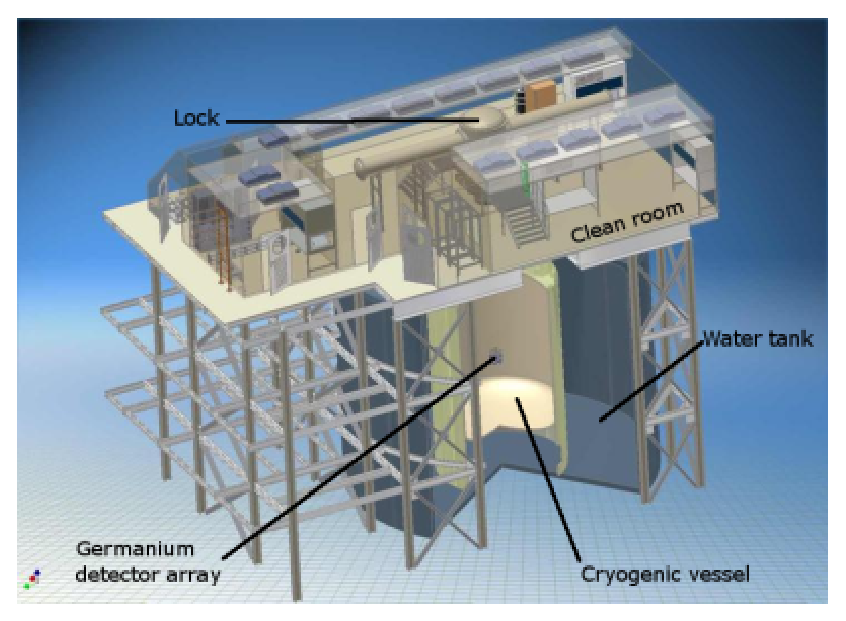
\includegraphics[width=0.7\textwidth]{gerda}  
  \caption{Schematic drawing of GERDA. A cryostat inside a water tank     is surrounded by a superstructure holding a cleanroom and lock     system.}
  \label{fig:gerda}
\end{figure}

\subsection{Location and muon veto}
\label{sec:gerda:loca}
In order to reduce the cosmic ray induced background GERDA is located in Hall A of the INFN Gran Sasso National Laboratory (LNGS), Italy. The LNGS is the largest underground facility in the world for low-background experiments. It is accessed from a 10~km long highway tunnel under the Gran Sasso mountains. It has three experimental halls hosting a large variety of experiments, most of which focus on dark matter or neutrino physics. Fig.~\ref{fig:lngs} shows the location of GERDA inside the LNGS. The main experimental site of GERDA is between the Large Volume Detector (LVD) and the service tunnel crossing Hall A. The GERDA auxiliary and cryogenic storage system will be located in the service tunnel on the northeast side of Hall A.

\begin{figure}[tbhp]
  \centering
  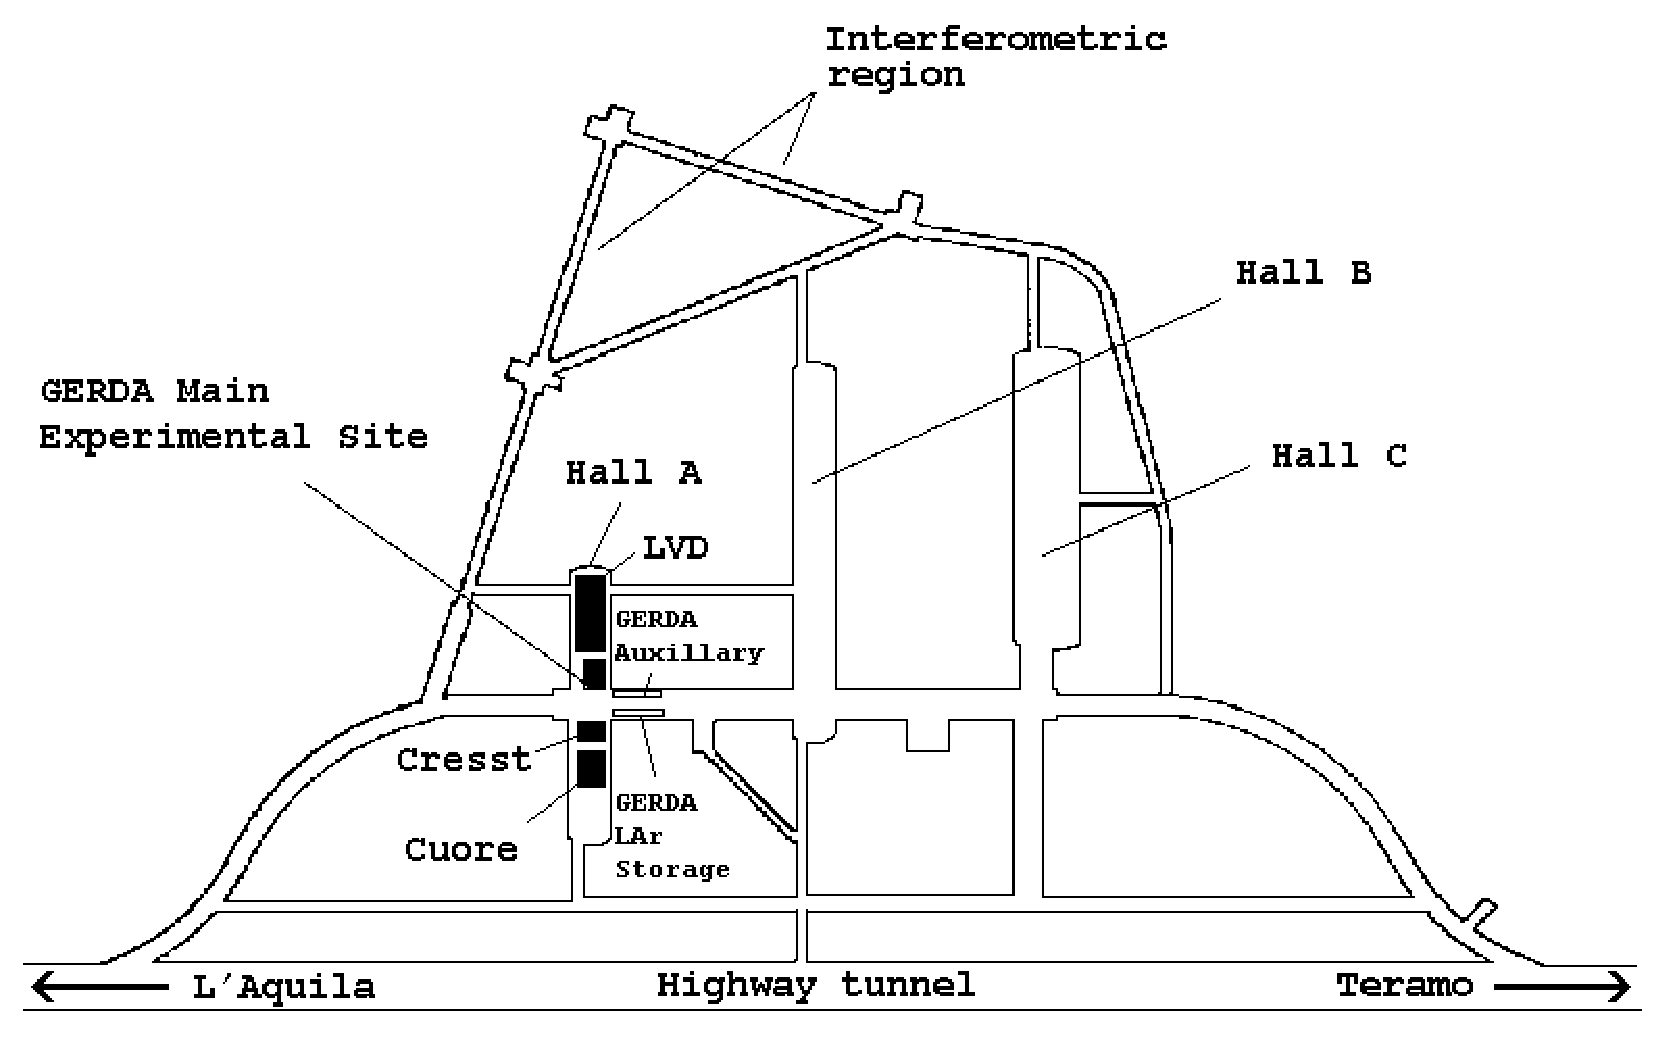
\includegraphics[width=0.8\textwidth]{lngs}  
  \caption{Location of GERDA at LNGS. The main experimental site of     GERDA is between the Large Volume Detector (LVD) and a service     tunnel crossing Hall A. The GERDA auxiliary and cryogenic storage     system will be located in the service tunnel on the northeast side     of Hall A.}
  \label{fig:lngs}
\end{figure}

The overburden of 1.4~km of rock on top of the experimental halls corresponds to 3400 meter of water equivalent (m.w.e). It reduces the cosmic ray induced muon (neutron) flux by a factor of $10^{6}$ ($10^{3}$) compared to the surface. The energy and angular distribution of cosmic ray muons in Hall A of LNGS have been precisely measured~\cite{Amb95, Lip91, Amb03}. A comprehensive study of cosmic ray induced muon and neutron background in underground laboratories can be found in Ref.~\cite{Mei06}.

In order to further reduce the muon induced background an additional muon veto system will be implemented. Cosmic muons traversing the water buffer will cause \u{C}erenkov radiation. To detect the radiation 66 photomultiplier tubes (PMTs) will be installed on the walls of the water tank. The positions of PMTs are optimized according to Monte Carlo simulation. Together with these PMTs the water tank is operated as a \u{C}erenkov detector. The detection efficiency is about 95\% depending on the incident angle of the muon. In order to compensate for the missing water volume around the neck of the cryostat plastic scintillator plates will be placed on top of the clean room. They are used to detect the muons entering the cryostat almost vertically. The combined detection efficiency is expected to be above 99\%.

\subsection{Water tank and cryostat}
\label{sec:gerda:rock}
To thermalize and absorb the neutron radiation from the rock $\sim 630$~m$^{3}$ of ultra-pure water will be filled in a stainless steel tank with an outer diameter of 10~m and a height of about 8~m. Since liquid argon can be produced with a much greater purity than lead or even copper traditionally used for shielding, a total of approximately 98~t of liquid argon will be stored in a cryostat placed inside the water tank to shield $\gamma$-rays from the rock and water. The vessel is made of stainless steel with an internal copper liner. The height of the vessel is 5.88~m (7.62~m with the neck) with an outer diameter of 4.16~m.

\subsection{Detector suspension system and electronics}
\label{sec:gerda:cable}
Germanium detectors will be lowered into liquid argon from the top of the cryostat. In order to minimize the radioactivity in the suspension system low mass copper frames, a novel contacting scheme and minimal cabling will be used (See Fig.~\ref{fig:array} left). The frames are made of thin ultra-pure copper bars with a total weight of about 30~g per detector. They will be chained vertically into strings. Each string consists of 3 detectors of the same type, as shown in the middle of Fig.~\ref{fig:array}. The whole detector array could maximally consists of 16 hexagonally packed detector strings as shown in Fig.~\ref{fig:array} right. 

The horizontal distance between the centers of two detectors is 9~cm. The vertical clearance between two detectors is about 6~cm. The Phase I detectors are p-type diodes with a cylindrical closed-ended coaxial geometry. The detectors are enriched in $^{76}$Ge to a level of about 86\% and have masses between 0.9~kg and 2.9~kg. The detectors for Phase II will be cylindrical true coaxial n-type diodes. The precise size of the detectors will depend on manufacturing details. The most likely dimensions are a height of 70~mm and a diameter of 75~mm. The detectors will be segmented 6-fold in the azimuthal angle $\phi$ and a 3-fold in the height z. 

\begin{figure}[tbhp]
  \centering
  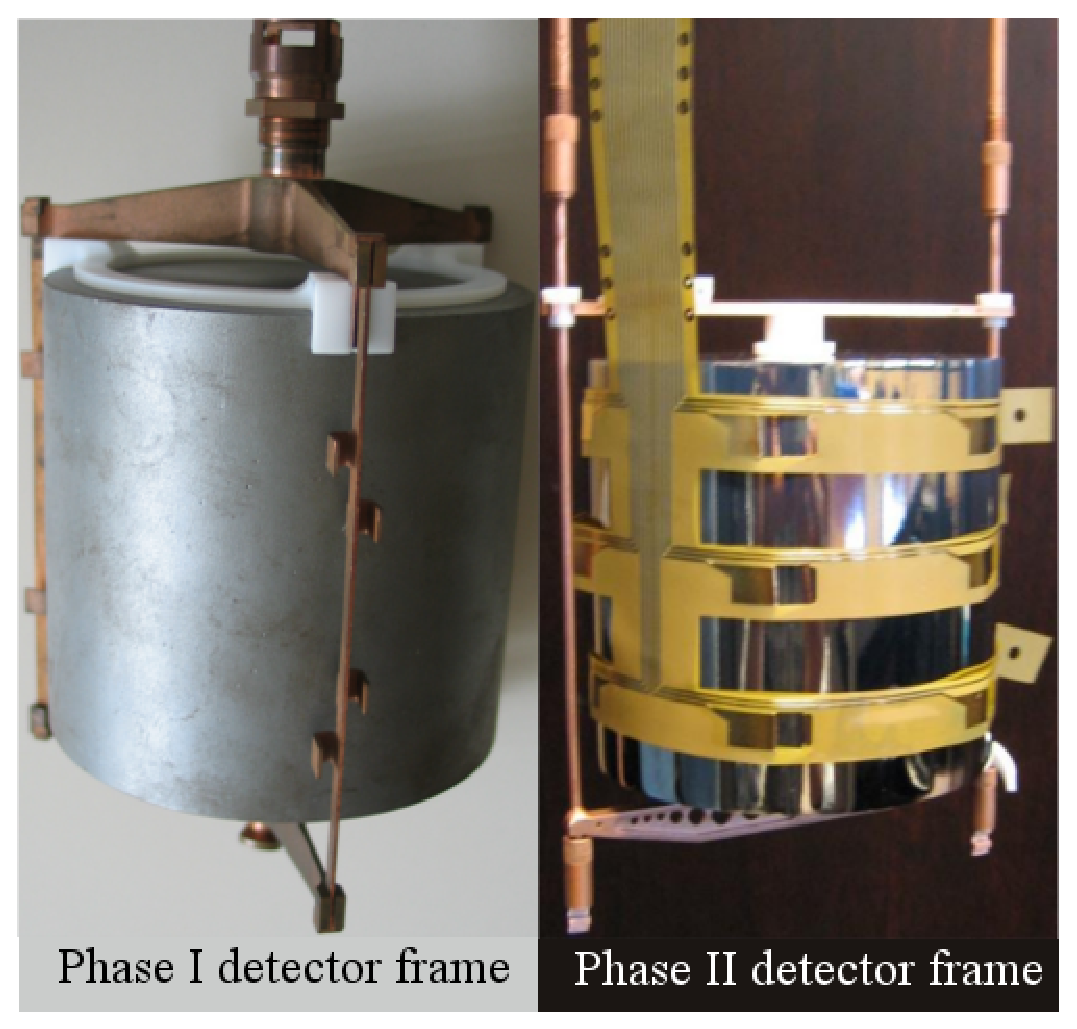
\includegraphics[width=0.33\textwidth]{detectorFrame}
  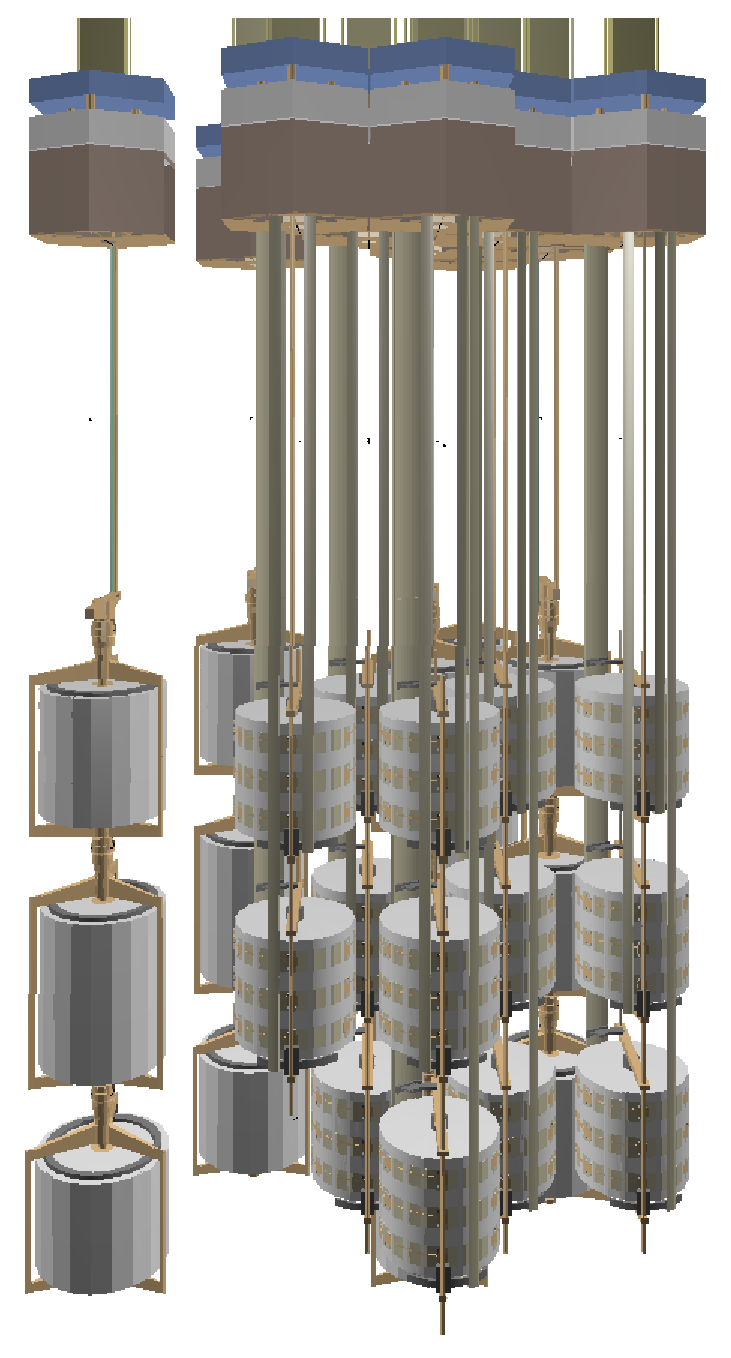
\includegraphics[width=0.2\textwidth]{array}   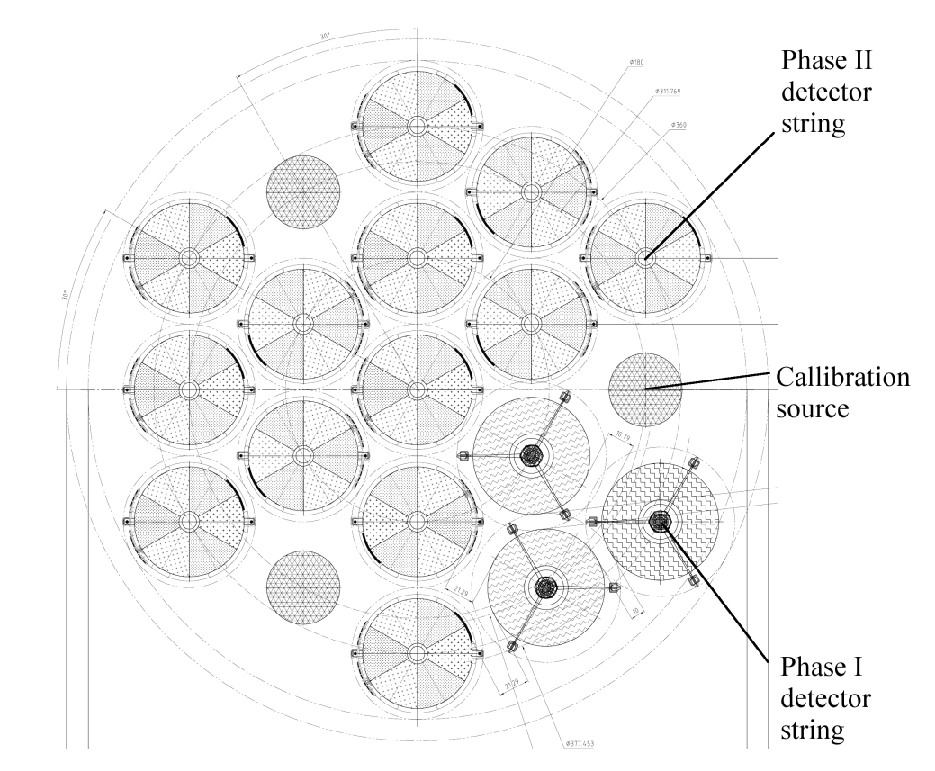
\includegraphics[width=0.45\textwidth]{arrayTop}
  \caption{Detector array configuration. The left plot shows single     Phase I detector with copper frame and Phase II detector with     copper frame and a novel contacting scheme. The middle plot shows     how the detectors are chained into strings and hung together in     liquid argon.  The right plot shows the top view of the full array     indicating the possible positions for the Phase I and Phase II     detector strings as well as for the calibration sources.}
  \label{fig:array}
\end{figure}

A couple of solutions are actively pursued for the read-out electronics of GERDA~\cite{Cat07}. A likely scheme foresees a cold FET close to the crystal followed by amplifying and load driving circuits located at room temperature. The cold FET would be placed near the connection matrix (top blocks in the middle plot of Fig.~\ref{fig:array}) 30~cm above the detector array. Pre-amplified signals would be sent to electronics located outside the lock system at room temperature through at least 6~m long cables.

\subsection{Detector storage and clean room}
\label{sec:gerda:source}
Whenever above ground, germanium detectors are exposed to cosmic radiation and radioactive isotopes are produced inside the detector through spallation caused by energetic cosmic rays. Two cosmogenic isotopes, $^{60}$Co and $^{68}$Ge, have Q-values above that of $^{76}$Ge $0\nu\beta\beta$ decay and are potential sources of background. Therefore the time above ground needs to be minimized. Since the half life time of $^{60}$Co and $^{68}$Ge is 5.3 years and 271 days, respectively, a passive method to reduce the contamination is to keep the detectors long enough underground and wait for it to decay.

When exposed to the air the surface a germanium detector can collect dust which contains many radioactive isotopes, particularly Pb$^{214}$, undergoing $\alpha$ decay. Some parts of the detector surface are not fully charge sensitive and only part of the energy lost by the $\alpha$ particle can be detected. This may result in a signal close to the $Q$-value of $^{76}$Ge $0\nu\beta\beta$ decay. Therefore the testing, preparation and insertion of the detector has to be done in a rather clean environment. For this purpose, a class 10000 clean room with radon-reduced air will be built on top of the cryostat. It houses a lock through which detector strings are inserted into and removed from the cryogenic volume. Detector handling will be performed in flow-boxes and a detector mounting station which will reach class 100.  The lock consists of a rail system which allows to move detector strings into their correct position and lower them into the cryostat. In addition, the clean room will be used to temporarily store germanium detectors under a controlled atmosphere of gaseous argon as shown in Fig.~\ref{fig:store}.

\begin{figure}[tbhp]
  \centering
  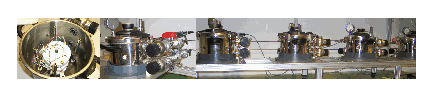
\includegraphics[width=\textwidth]{storage}
  \caption{Detector storage system. The left picture shows an open     vacuum pot with a detector inside. The middle picture shows a     closed vacuum pot equipped with valves and gas flux sensor. The     right picture shows four vacuum pots connected with gas tubes.}
  \label{fig:store}
\end{figure}

\subsection{Other background rejection techniques}
\label{sec:gerda:anti}
Other background rejection techniques to be used in GERDA include (1) anti-coincidence requirement, (2) pulse shape analysis, and (3) instrumentation of the cryostat.
\begin{description}
\item[Anti-coincidence:] Compton-scattered photons are likely to   deposit energy in more than one detector while $0\nu\beta\beta$   decay electrons will predominantly deposit energy in only one   detector. Photons can thus be identified by requiring more than one   detector to see energy above the threshold. Considering the   segmented detectors for Phase II photons depositing energy in one   crystal can still be identified by requiring more than one segment   to show energy. Time anti-coincidence vetos could also be used to   reject background induced by the decay of $^{68}$Ge and $^{77}$Ge   meta stable state. Feasibility studies are currently carried out.
\item[Pulse shape analysis:] Although photons are likely to create   more than one energy deposition, they could all be in one segment;   the anti-coincidence between segments cannot distinguish this kind   of event from a $0\nu\beta\beta$ decay. However, by analyzing   the time structure of the detector response, \textit{i.e.} pulse   shape, photon induced events can still be identified~\cite{Kev07}.
\item[Instrumentation of the cryostat:] Liquid argon scintillates if   energy is deposited inside the argon volume. The scintillation light   can be detected by PMT's mounted on the walls of the cryostat.   Events with photons in the final state which deposit only a fraction   of their energy inside the germanium detectors can be vetoed by   requiring an anti-coincidence between the observed scintillation   light and the energy deposit inside the detectors.  This technique   is not part of the GERDA baseline design. Feasibility studies are   currently being performed~\cite{Pei05, Orr06}.
\end{description}

\section{Status}
\label{sec:gerda:stat}
This section closes with the status of GERDA as of Winter 2008/09. Important milestones are discussed below.  

\subsection{Cryostat and water tank}
\label{sec:gerda:stat1}
On 6 March 2008, the cryostat was delivered to LNGS and placed at the foreseen location in Hall A (see Fig.~\ref{fig:cryo} center). Mounting of the internal copper shield was completed on March 18. The cryostat underwent pressure tests, helium leak tests, liquid nitrogen evaporation tests and radon emanation measurements. The water tank installation finished at the end of June (see Fig.~\ref{fig:cryo}right). The installation of the cryostat and water tank are major milestones for GERDA.

\begin{figure}[tbhp]
  \centering
  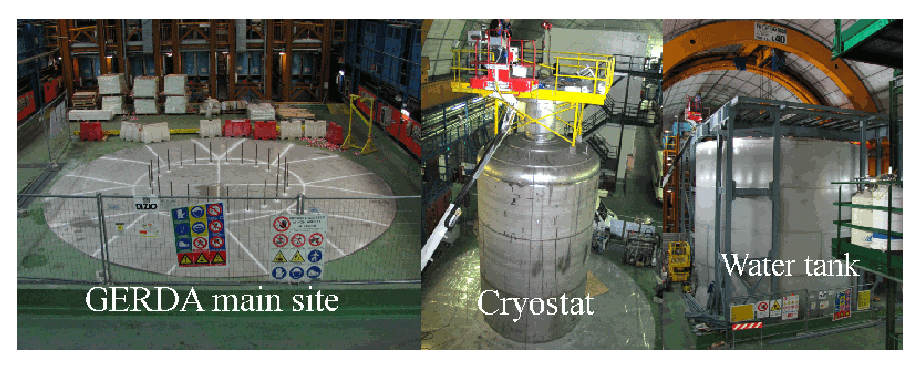
\includegraphics[width=\textwidth]{cryostat}
  \caption{Construction of cryostat and water tank at the GERDA main     site.  From left to right: the empty GERDA main site, the     installed cryostat, the water tank and superstructure around it.}
  \label{fig:cryo}
\end{figure}

\subsection{Clean room and lock system}
\label{sec:gerda:stat2}
The right picture of Fig.~\ref{fig:cryo} shows the first parts of the superstructure around the water tank, on top of which the clean room and lock will be built. The design of the clean room is finished. The construction is scheduled to finish in February 2009. The design of the complete lock structure is almost finished. The lock will be preinstalled at the Max-Planck-Institut f\"ur Physik in Munich and then transported to the LNGS in 2009. A provisional lock system is in production. It will be used before the complete lock system is ready so that the commissioning of GERDA can start at February 2009.

\subsection{Phase I and II detectors}
\label{sec:gerda:stat3}
In total 17.9~kg of enriched and 15~kg of non-enriched high-purity p-type germanium detectors from IGEX, HdM and the Genius Test Facility (GTF)~\cite{Kla02} will be operated in Phase I of GERDA. Stability tests of the operation of p-type detectors in cryogenic liquids are practically completed. 

A total of 37.5~kg of enriched germanium was procured for GERDA Phase II detectors. It has an enrichment level of about 90\% and is stored in the HADES facility in the form of GeO$_{2}$. The purification tests with depleted germanium have shown that the yield is about 90\%, and the exposure time above ground will not exceed $2 \sim 3$ days. The resulting 6N material will be transformed into crystals by the Institut f\"ur Kristallz\"uchtung (IKZ) in Berlin. Crystals with a concentration of impurities between $10^{12}$ and $10^{11}$ per cm$^{3}$ has been pulled at IKZ, see Fig.~\ref{fig:pulling}. The \u{C}zochralski puller has been refurbished to produce larger crystals.
\begin{figure}[tbhp]
  \centering
  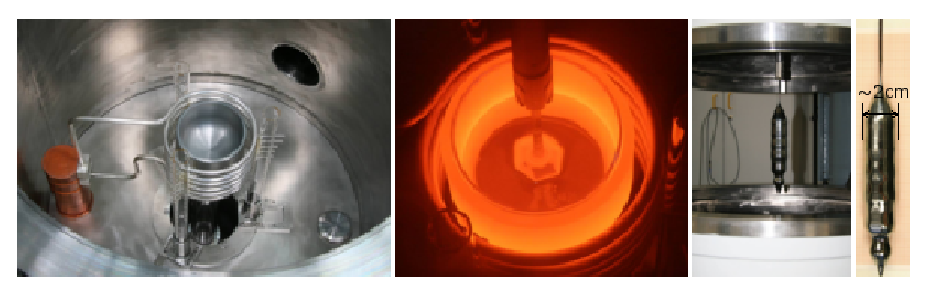
\includegraphics[width=\textwidth]{crystalPulling}
  \caption{From left to right: \u{C}zochralski puller, crystal being pulled, crystal above crucible and close-up of crystal.}
  \label{fig:pulling}
\end{figure}

Several Phase II prototype detectors were produced from natural germanium crystals. The detectors were produced by Camberra France who procured the crystals from Umicore. The first Phase II prototype detector operated in a conventional cryostat has been tested and characterized~\cite{Sie07}. The second prototype detector was operated in liquid nitrogen for months. The handling, operating and testing of the prototype detectors and the physics analysis based on the data from them are the main topics of this thesis and will be discussed in detail in the following chapters.


\section{Sensitivity}
\label{sec:gerda:sens}
A dedicated discussion about the sensitivity of GERDA can be found in Ref.~\cite{Cal06}. The left plot in Fig.~\ref{fig:gerda:limit} taken from Ref.~\cite{Cal06} shows the expected 90\% probability lower limit on the half lifetime of $0\nu\beta\beta$ decay versus the exposure under different background conditions. Also shown is the half lifetime for the claimed observation by H. V. Klapdor-Kleingrothaus \textit{et   al.}~\cite{Hei04}. The right plot shows the expected 90\% probability upper limit on the effective Majorana neutrino mass versus the exposure under different background conditions. The effective Majorana neutrino mass for the claimed observation is also shown. All mass values are determined from the half lifetime using the matrix elements reported in Ref~\cite{Rod07}.
\begin{figure}[tbhp]
  \centering
  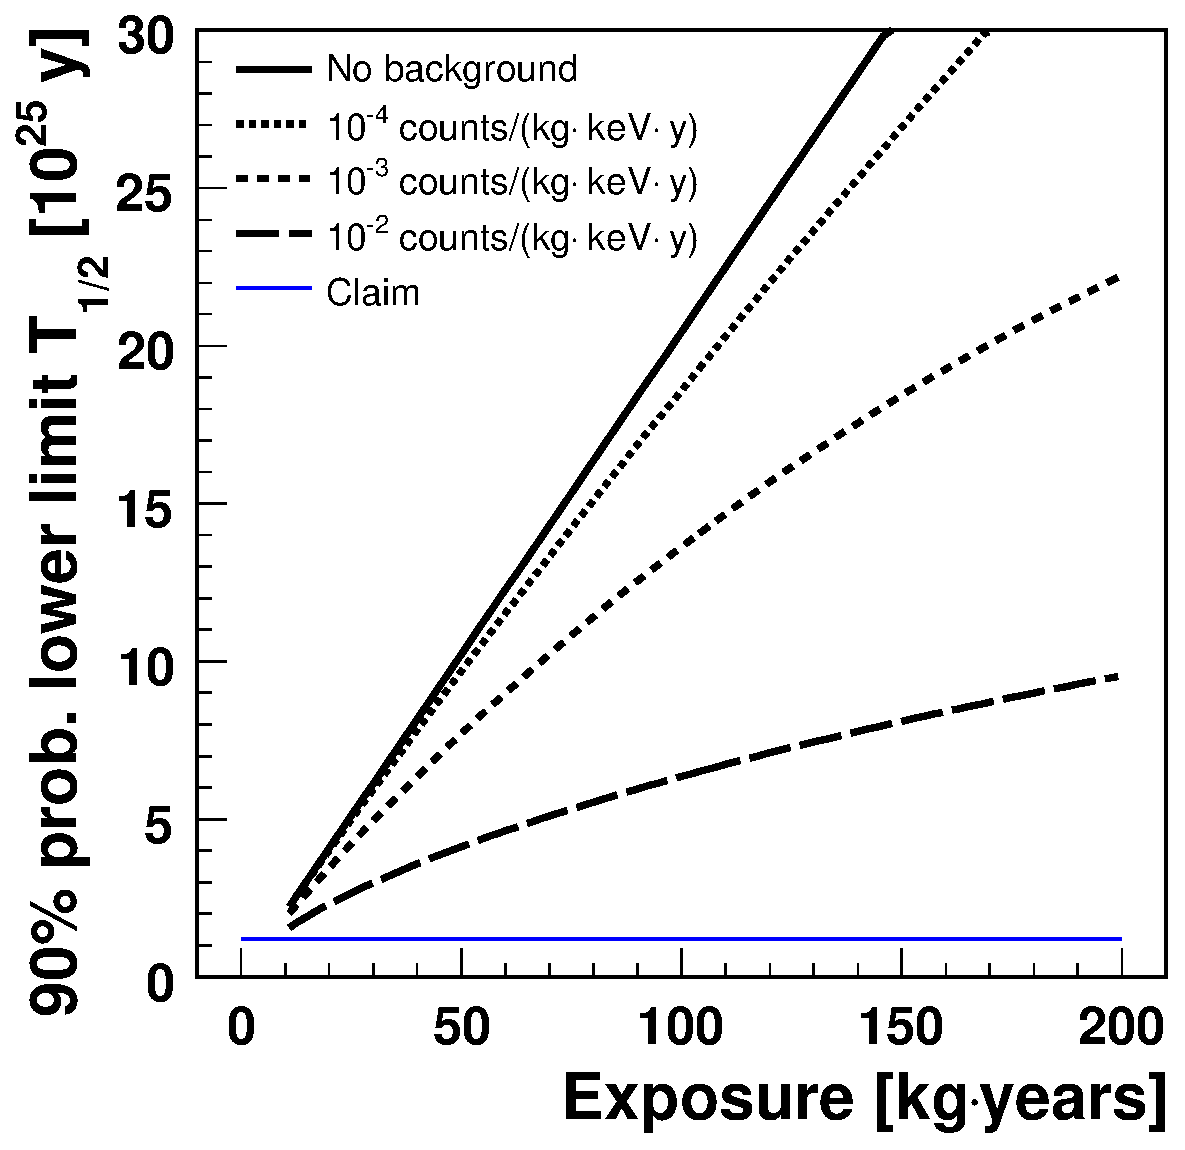
\includegraphics[width=0.45\textwidth]{limit_halflife}  \hfil
  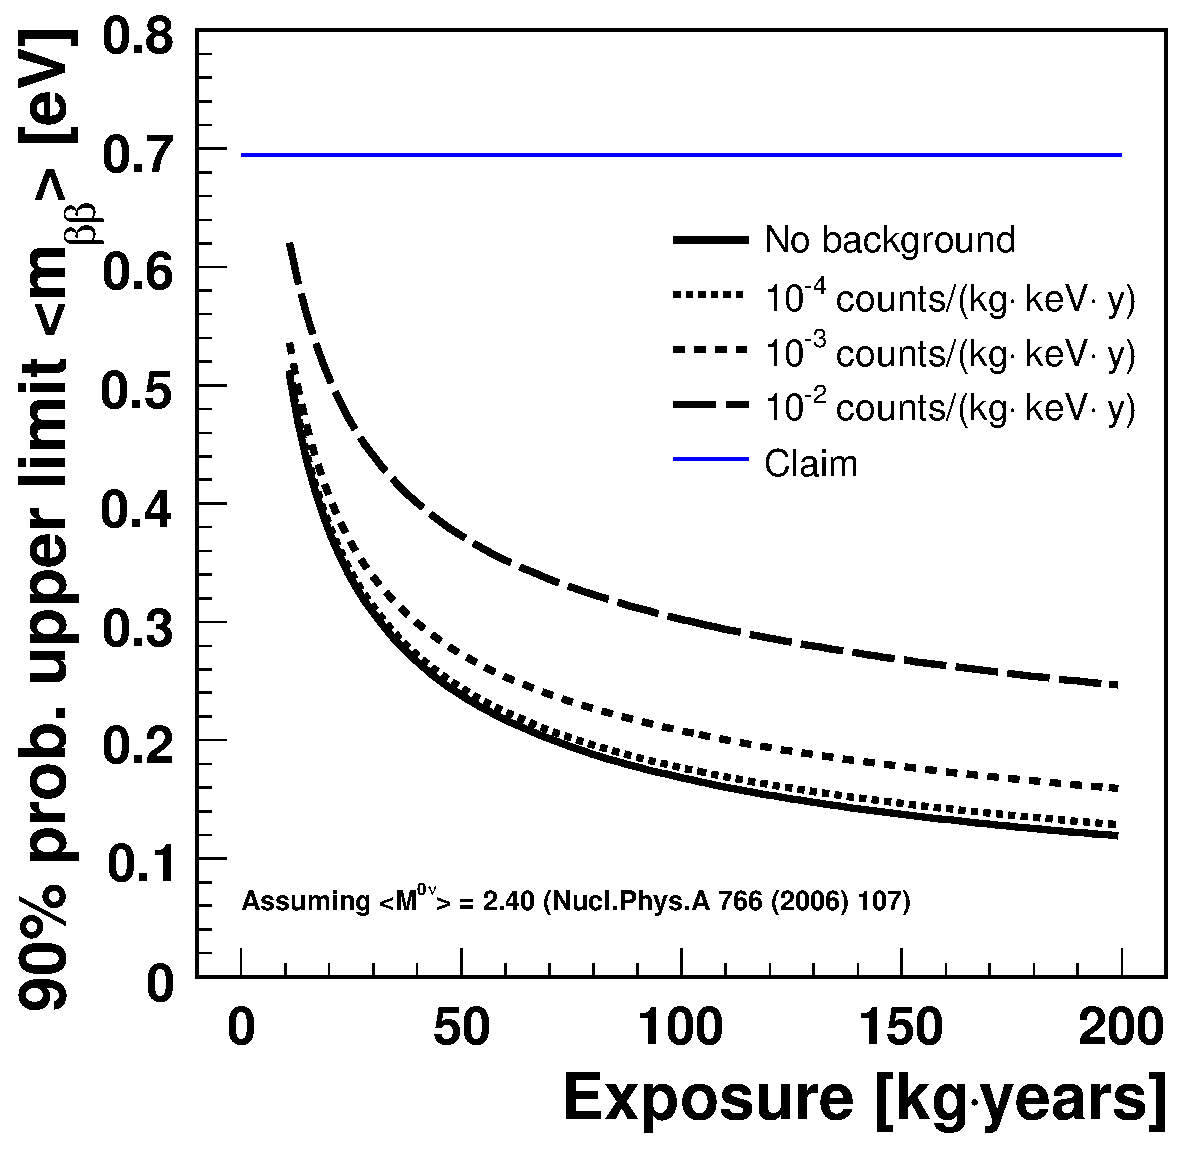
\includegraphics[width=0.45\textwidth]{limit_mass}
  \caption{The expected 90\% probability lower limit on the half     lifetime for $0\nu\beta\beta$ decay (left) and the expected 90\%     probability upper limit on the effective Majorana neutrino mass     (right) versus the exposure under different background conditions.     Also shown is the half lifetime and the effective Majorana     neutrino mass for the claimed observation by H. V.     Klapdor-Kleingrothaus \textit{et al.}~\cite{Hei04}. All mass     values are determined from the half lifetime using the matrix     elements reported in Ref~\cite{Rod07}.}
  \label{fig:gerda:limit}
\end{figure}

For GERDA Phase I, assuming a background level of $10^{-2}$~events/(kg$\cdot$keV$\cdot$year) and an exposure of
100~(kg$\cdot$year), an upper limit on $m_{\beta\beta}$ of
0.3~eV would be achievable. For Phase II, assuming a background level of $10^{-3}$~events/(kg$\cdot$keV$\cdot$year) and an exposure of
100~(kg$\cdot$year), an upper limit on $m_{\beta\beta}$ of
0.2~eV would be achievable.


%%% Local Variables:
%%% mode:latex
%%% TeX-master: "thesis"
%%% End:
